%instructs Latex to typeset the document as an article
%with a base font size of twelve points, and to produce
%a layout suitable for double sided printing on A4 paper
\documentclass [a4paper,twoside,12pt]{article}

%list package use
\usepackage{graphicx} %this one is for graphic
\usepackage{hyperref}

%define the title
\author{Quoc Anh Doan}
\title{Who is Richard Feynman?}

\begin{document}

%generates the title
\maketitle

%insert the table of contents
\tableofcontents
\section{Introduction}
An introduction about this man.
\section{Reason}
Reason why I did this.
\section{Reference}
References.
\newpage

See the Figure \ref{fig:feynman} for Feynman's picture 
	
"Richard Phillips Feynman (May 11, 1918 – February 15, 1988; IPA: /ˈfaɪnmən/) was an American physicist known for expanding the theory of quantum electrodynamics, the physics of the superfluidity of supercooled liquid helium, and particle theory. For his work on quantum electrodynamics, Feynman was a joint recipient of the Nobel Prize in Physics in 1965, together with Julian Schwinger and Shin-Ichiro Tomonaga; he developed a widely-used pictorial representation scheme for the mathematical expressions governing the behavior of subatomic particles, which later became known as Feynman diagrams" \cite{wiki}.


\begin{figure}[t]
  \begin{center}
    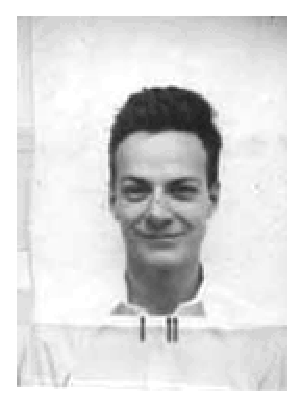
\includegraphics[width=0.5\textwidth]{graph}
    \caption{Richard Feynman}
    \label{fig:feynman}
  \end{center}
\end{figure}

\newpage

\begin{math}
s= \int (\frac{dx}{dt})^2 dt
\end{math}

\newpage
\begin{thebibliography}{9}
 

 
\bibitem{wiki}
\url{http://en.wikipedia.org/wiki/Richard_Feynman}
 on 04/04/2008.



\end{thebibliography}

%\ref{label:wiki}
%\usepackage[all]{hypcap}
%\ldots{} print elipse

\end{document}
